\documentclass[10pt, oneside]{article} 
\usepackage{amsmath, amsthm, amssymb, calrsfs, wasysym, verbatim, bbm, color, graphics, geometry}
\usepackage{graphicx}
\usepackage{float}
\usepackage{longtable}
\usepackage{rotating}
\usepackage{adjustbox}
\usepackage{booktabs}
\usepackage{caption}
\usepackage[english]{babel}
\usepackage[utf8]{inputenc}
\usepackage[table]{xcolor}
\usepackage{multicol}
\usepackage{hyperref}

\geometry{tmargin=.75in, bmargin=.75in, lmargin=.75in, rmargin = .75in}  

\newcommand{\R}{\mathbb{R}}
\newcommand{\C}{\mathbb{C}}
\newcommand{\Z}{\mathbb{Z}}
\newcommand{\N}{\mathbb{N}}
\newcommand{\Q}{\mathbb{Q}}
\newcommand{\Cdot}{\boldsymbol{\cdot}}

\newtheorem{thm}{Theorem}
\newtheorem{defn}{Definition}
\newtheorem{conv}{Convention}
\newtheorem{rem}{Remark}
\newtheorem{lem}{Lemma}
\newtheorem{cor}{Corollary}


\title{Computing Infrastructure: [Course Code]}
\author{[Sofia Martellozzo]}
\date{Academic Year 2021-2022}

\begin{document}

\maketitle
\newpage
\tableofcontents

\vspace{.25in}
\newpage

\section{Computing Infrastructure}

\subsection{Introduction}
\begin{defn}
{\bf Computing Infrastructure}: Technological infrastructure that provides hardware and software for computation to other systems and services.
\end{defn}


\begin{figure}[H]
    \begin{center}
    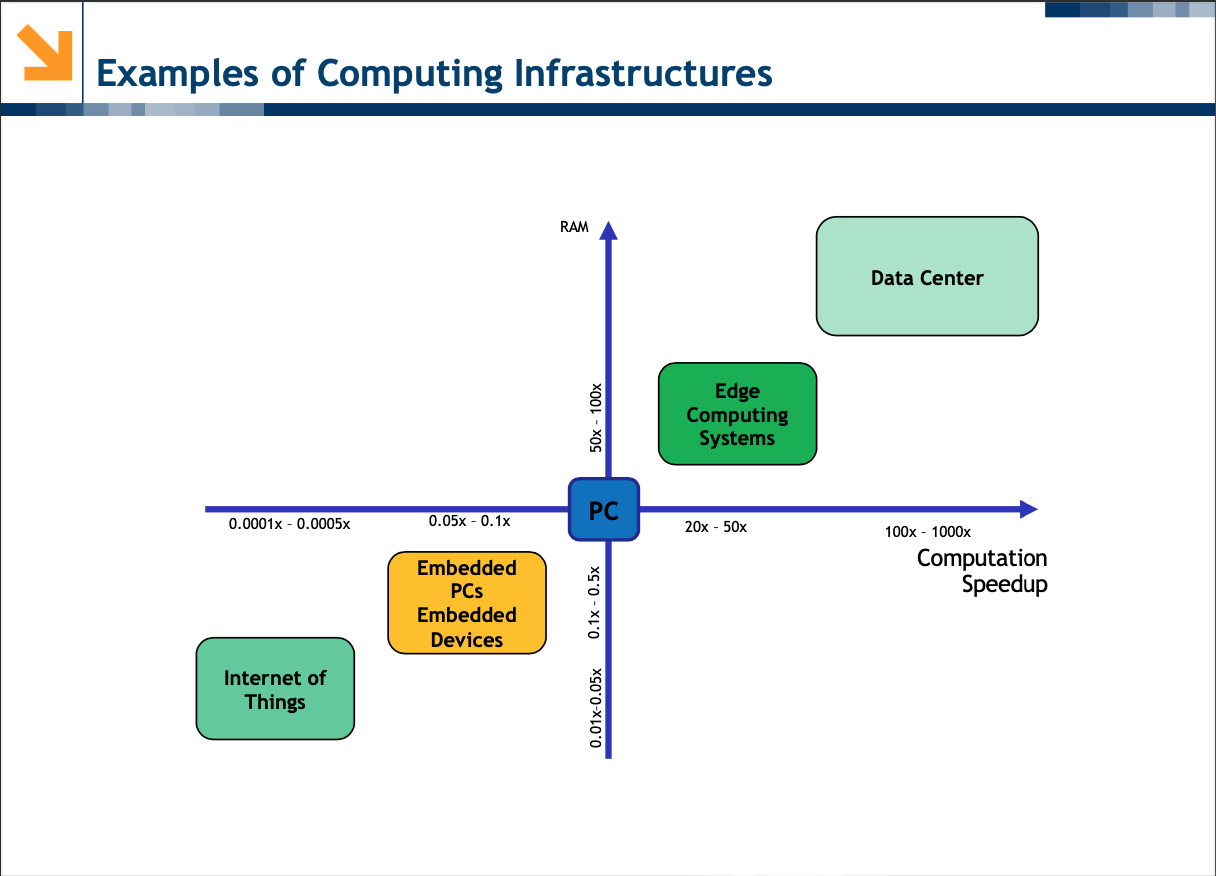
\includegraphics[width=0.5\textwidth]{img/img1.png}
    \caption{Computing Infrastructure}
    \label{fig:computing infrastructure}
    \end{center}
\end{figure}

\begin{multicols}{2}
\noindent
{\bf Advantages}:
\begin{itemize}
    \item Lower IT costs
    \item High performance
    \item Instant software updates
    \item “Unlimited” storage capacity
    \item Increased data reliability
    \item Universal document access
    \item Device Independence 
\end{itemize}

\columnbreak
\noindent
{\bf Disadvantages}:
\begin{itemize}
    \item Require a constant Internet connection
    \item Do not work well with low-speed connections
    \item Hardware Features might be limited
    \item Privacy and security issues
    \item High Power Consumption (1\% overall worldwide total energy consumption due to datacenters)
    \item Latency in making decision
\end{itemize}

\end{multicols}


\begin{figure}[H]
    \begin{center}
    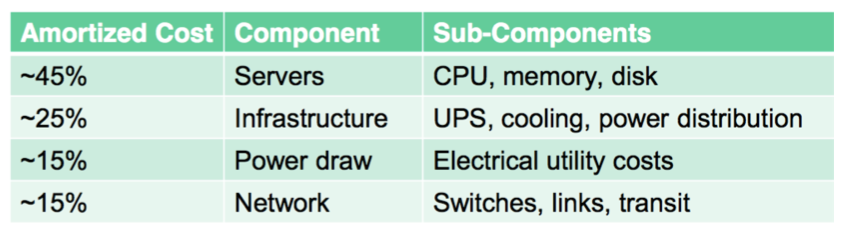
\includegraphics[width=0.5\textwidth]{img/img2.png}
    \label{fig:consumptions}
    \end{center}
\end{figure}

\newpage

%------------------------------------------------------%
\section{Data WareHouse}

\subsection{Introduction}
In the last few decades, computing and storage have moved from PC- like clients to smaller, often mobile, devices, combined with large internet services.\\
Traditional enterprises are also shifting to Cloud computing.
\begin{figure}[H]
    \begin{center}
    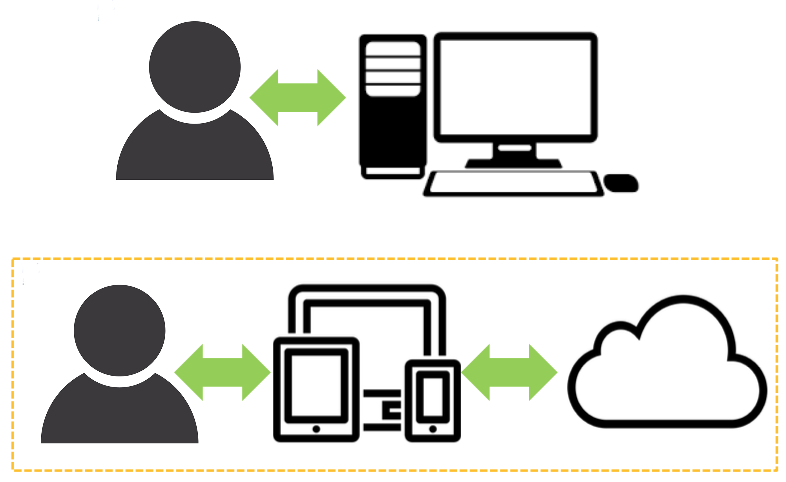
\includegraphics[width=0.5\textwidth]{img/img3.png}
    \label{fig:computing and storage}
    \end{center}
\end{figure}

\begin{multicols}{3}
\noindent
{\bf User experience improvements}
\begin{itemize}
    \item Ease of management (no configuration or backups needed)
    \item Ubiquity of access
\end{itemize}

\columnbreak
\noindent
{\bf Advantages to vendors}
\begin{itemize}
    \item Software-as-a-service allows faster application development (easier to make changes and improvements)
    \item Improvements and fixes in the software are easier inside their data centers (instead of updating many millions of clients with peculiar hardware and software configurations)
    \item The hardware deployment is restricted to a few well-tested configurations.
\end{itemize}

\columnbreak
\noindent
{\bf Server-side computing allows}
\begin{itemize}
    \item Faster introduction of new hardware devices (e.g., HW accelerators or new hardware platforms)
    \item Many application services can run at a low cost per user.
\end{itemize}

\end{multicols}
Some workloads require so much computing capability that they are a more natural fit in datacenter (and not in client-side computing).\\
A couple of examples (Search services (web, images, and so on), Machine and Deep Learning (\href{https://www.theguardian.com/commentisfree/2020/sep/08/robot-wrote-this-article-gpt-3}{GPT-3}).

\subsection{From Data Centers to Warehouse-scale computers}
{\bf Data centers} = is a place in which there are many servers\\
{\bf Whareouse} = is a type of Data Center, it works as a computer.\\
The trends toward server-side computing and widespread internet services created a new class of computing systems:
\begin{defn}
{\bf warehouse-scale computers (WSCs)}The massive scale of the software infrastructure, data repositories, and hardware platform.
\begin{itemize}
    \item is an internet service (= service provided by inyternet)
    \item may consist of tens or more individual programs (= not a single program, a collection of them that together create/provide the service)
    \item such programs interact to implement complex end-user services such as email, search, maps or machine learning.
\end{itemize}
\end{defn}
Data centers are buildings where multiple servers and communication units are co-located because of their common environmental requirements and physical security needs, and for ease of maintenance.\\
In {\bf Traditional Data Center}: typically host a large number of relatively small- or medium-sized applications, each applications is running on a dedicated hardware infrastructure that is de-coupled and protected from other systems in the same facility, applications tend not to communicate each other. Those data centers host hardware and software for multiple organizational units or even different companies.
\begin{figure}[H]
    \begin{center}
    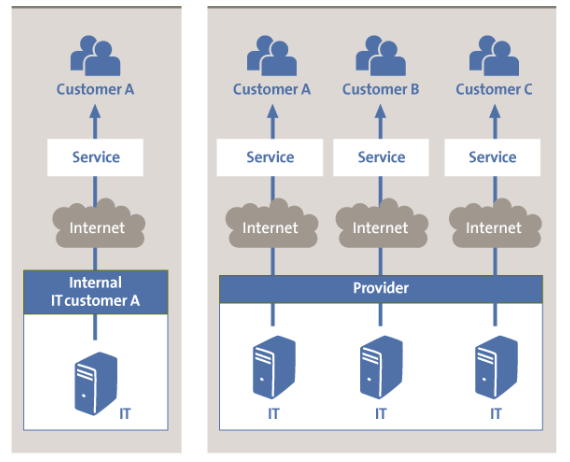
\includegraphics[width=0.3\textwidth]{img/img4.png}
    \caption{Traditional Data Center}
    \label{fig:Traditional Data Center}
    \end{center}
\end{figure}
{\bf WSCs} belong to a single organization, use a relatively homogeneous hardware and system software platform (=> easier to manage and cheaper, but has limitations on functionalities), and share a common systems management layer (such as Google, Facebook, Alibaba, Amazon, Dropbox...).\\
(you have 1 services that you want to provide to a 'huge' amount of customers)\\
Run a smaller number of very large applications (or internet services).\\
The common resource management infrastructure allows significant deployment flexibility.\\
The requirements of:
\begin{itemize}
    \item homogeneity
    \item single-organization control
    \item cost efficiency
\end{itemize}
\begin{figure}[H]
    \begin{center}
    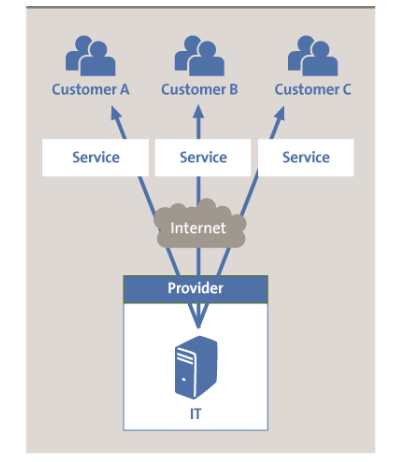
\includegraphics[width=0.25\textwidth]{img/img5.png}
    \caption{Warehouse-Scale Computers}
    \label{fig:WSCs}
    \end{center}
\end{figure}
Initially designed for online data-intensive web workloads, WSCs also now power public clouds computing systems (e.g., Amazon, Google, Microsoft). Such public clouds do run many small applications, like a traditional data center. (All of these applications rely on Virtual Machines (or Containers), and they access large, common services for block or database storage, load balancing, and so on, fitting very well with the WSC model).\\
These are not just a collection of servers: \\The software running on these systems executes on clusters of hundreds to thousands of individual servers (far beyond a single machine or a single rack)\\
+ \\The machine is itself this large cluster or aggregation of servers and needs to be considered as a single computing unit. (=$>$ scale up in terms of performance)\\
{\bf Several data-centers}:
Multiple Data Center located far apart (placed near point of interest) => becomes important also the PRIVACY: data of a country must remain in it.\\
Multiple data centers are (often) replicas of the same service (to reduce user {\bf latency} and improve serving {\bf throughput}).\\
A request is typically fully processed within one data center.\\
{\bf Availability}:
Services provided through WSCs must guarantee high availability, typically aiming for at least 99.99\% uptime (i.e., one-hour downtime per year). Achieving such fault-free operation is difficult when a large collection of hardware and system software is involved.\\
WSC workloads must be designed to gracefully tolerate large numbers of component faults with little or no impact on service level performance and availability.

\subsection{Architectural Overview of WSCs}
Hardware implementation of WSCs might differ significantly each other; However, the architectural organization of these systems is relatively stable.
\begin{multicols}{2}
\begin{figure}[H]
    \begin{center}
    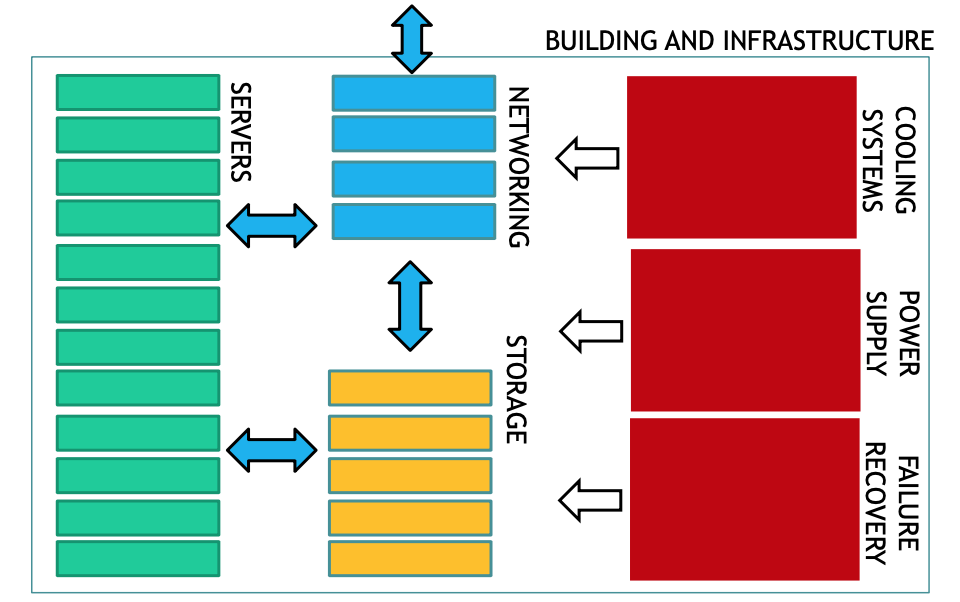
\includegraphics[width=0.4\textwidth]{img/img6.png}
    \caption{Warehouse-Scale Computers Overview}
    \label{fig:WSCs overview}
    \end{center}
\end{figure}
\columnbreak
\begin{figure}[H]
    \begin{center}
    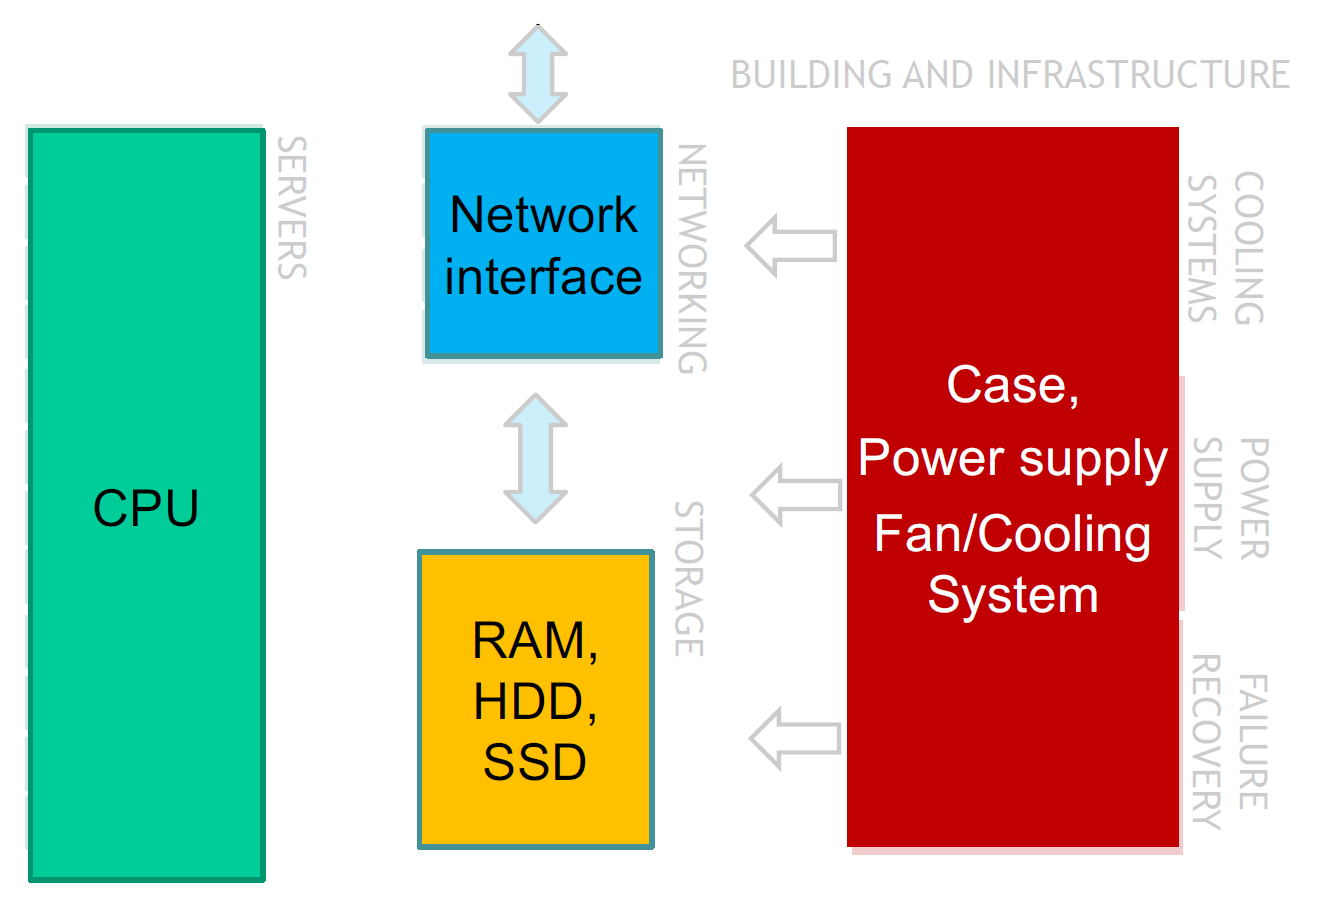
\includegraphics[width=0.4\textwidth]{img/img7.png}
    \caption{}
    \label{fig:WSCs overview2}
    \end{center}
\end{figure}
\end{multicols}

\begin{itemize}
    \item \color{green}\textbf{Servers}\color{black}
    : the main processing equipment
    
    \item \color{yellow}\textbf{Storage}\color{black}
    : how and where to store the information
    \item \color{blue}\textbf{Networking}\color{black}
    : providing internal and external connections
    \item \color{red}\textbf{Building and Infrastructure}\color{black}
    :WSC has other important components related to power delivery, cooling, and building infrastructure that also need to be considered
\end{itemize}




%------------------------------------------------------%
\newpage
\section{Server}
\subsection{Overview}
Servers hosted in individual shelves are the basic building blocks of WSCs. They are interconnected by hierarchies of networks, and supported by the shared power and cooling infrastructure. They are stored in  shelves called wraks, that are organized along corridors. All servers are connected to each other in the same wrak, but also (on a higher level) communicate through different wrack.
 They have 3 type of shape:
    \begin{itemize}
        \item Rack (1U or more)
        \item Blade enclosure format 
        \item Tower
    \end{itemize} 
    They may differ in: 
    \begin{itemize}
        \item Number and type of CPUs.
        \item Available RAM Locally attached disks (HDD, SSD or not installed).
        \item Other special purpose devices (like GPUs, DSPs and coprocessors).
    \end{itemize}  
and are usually built in a tray or blade enclosure format, housing the motherboard, chipset, additional plug-in components.

\subsubsection{The Motherboard}
The motherboard provides sockets and plug-in slots to install CPUs, memory modules (DIMMs), local storage (such as Flash SSDs or HDDs), and network interface cards (NICs) to satisfy the range of resource requirements.
\subsubsection{Chipset and additional components}
\begin{itemize}
    \item Number and type of CPUs:
\begin{itemize}
    \item From 1 to 8 CPU socket
    \item Intel Xeon Family, AMD EPYC, etc..
\end{itemize}
    \item Available RAM
    \begin{itemize}
        \item From 2 to 192 DIMM Slots
    \end{itemize}
    \item Locally attached disks:
    \begin{itemize}
        \item From 1 to 24 Drive Bays
        \item HDD or SSD (see specific lecture)
        \item SAS (higher performance but more expensive) or SATA (for entry level servers, usually cheaper)
    \end{itemize}
    \item Other special purpose devices:
    \begin{itemize}
        \item From 1 to 20 GPUs per node, or TPUs
        \item NVIDIA Pascal, Volta, etc..
    \end{itemize}
    \item Form factor:
    \begin{itemize}
        \item Form 1U to 10U
        \item Tower
    \end{itemize}
\end{itemize}
We distinguish between rack, tower and blade.

\subsubsection{Rack}
Racks are special shelves that accommodate all the IT equipment and allow their interconnection. The rack are used to store many {\bf Rack server}.\\ 
IT equipment must conform to specific sizes to fit into the rack shelves. Them has different hight, but same SIZE, that is {\bf standardize} (so make them easier to design): server racks are measured in rack units "U's".\\ The advantages of using these racks is that it allows designers to stack up (one on top of the others) other electronic devices along with the servers.\\
\newline
A Rack is not only a physical structure:
\begin{multicols}{2}
\noindent
\begin{figure}[H]
    \begin{center}
    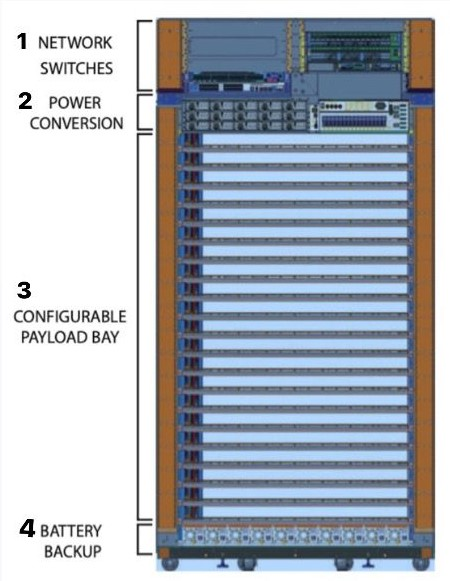
\includegraphics[width=0.4\textwidth]{img/img8.jpeg}
    \caption{RACK Servers}
    \label{fig:RACK servers}
    \end{center}
\end{figure}
\columnbreak
\noindent
(3) The rack is the shelf that holds tens of servers together. \\(2-4) It handles shared power infrastructure, including power delivery, battery backup, and power conversion.\\
(2) There are 2 types of electronic delivery: it can provide/automatically select the server (can swich ON and OFF remotely the servers).\\
(4) It is used in case of problems with energy (power failure):
\begin{itemize}
    \item just swich off if a power failure occur, them cannot supply all the power demand (execution)
    \item it provides 15 minutes of power, that is the time to swich on the power supply generator (source) 
\end{itemize}
(3) The width and depth of racks vary across WSCs: some are classic 19-in wide, 48-in deep racks, while others can be wider or shallower.\\ 
(1) It is often convenient to connect the network cables at the top of the rack, such a rack-level switch is appropriately called a Top of Rack (TOR) switch.
\end{multicols}

Rack servers:\\
It is designed to be positioned in a bay, by vertically stacking servers one over the another along with other devices
\begin{multicols}{2}
\noindent
{\bf \color{green}Pros}\color{black}
\begin{itemize}
    \item {\bf Failure containment}: very little effort to identify, remove, and replace a malfunctioning server with another.
    \item {\bf Simplified cable management}: easy
and efficient to organize cables.
    \item {\bf Cost-effective}: Computing power and efficiency at relatively lower costs.
\end{itemize}
\columnbreak
\noindent
{\bf \color{red}Cons}\color{black}
\begin{itemize}
    \item {\bf Power usage}: Needs of additional cooling systems due to their high overall component density, thus consuming more power.
    \item {\bf Maintenance}: Since multiple devices are placed in racks together, maintaining them gets considerably tough with the increasing number of racks.
\end{itemize}
\end{multicols}
\newpage
\subsubsection{Tower}
It is the simplest but is not usually adopted.
\textbf{Tower Servers}
look and feel a lot like traditional tower PCs.
Like everything they have their Pros and Cons.
\begin{multicols}{2}
\noindent
{\bf \color{green}Pros}\color{black}
\begin{itemize}
    \item {\bf Scalability and ease of upgrade}: customized and upgraded based on necessity.
    \item {\bf Cost-effective}: Tower servers are probably the cheapest of all kinds of servers
    \item {\bf Cools easily}: Since a tower server has a low overall component density, it cools down easily.
\end{itemize}
\columnbreak
\noindent
{\bf \color{red}Cons}\color{black}
\begin{itemize}
    \item {\bf Consumes a lot of space}: These servers are difficult to manage physically.
    \item {\bf Provides a basic level of performance}: a tower server is ideal for small businesses that have a limited number of clients.
    \item {\bf Complicated cable management}: devices aren't easily routed together
\end{itemize}
\end{multicols}

  
\subsubsection{Blade}
Blade servers are the latest and the most advanced type of servers in the market. They can be termed as hybrid rack servers (like orizontal rack server but placed vertically), in which servers are placed inside blade enclosures, forming a blade system. The biggest advantage of blade servers is that these servers are the smallest types of servers available at this time and are great for conserving space. A blade system also meets the IEEE standard for rack units and each rack is measured in the units of “U’s”.
\begin{multicols}{2}
\noindent
{\bf \color{green}Pros\color{black}}
\begin{itemize}
    \item {\bf Load balancing and failover}: Thanks to its much simpler and slimmer infrastructure, load balancing among the servers and failover management tends to be much simpler.
    \item {\bf Centralized management}: In a blade server, you can connect all the blades through a single interface, making the maintenance and monitoring easy.
    \item {\bf Cabling}: Blade servers don't involve the cumbersome tasks of setting up cabling. Although you still might have to deal with the cabling, it is near to negligible when compared to tower and rack servers.
    \item {\bf Size and form-factor}: They are the smallest and the most compact servers, requiring minimal physical space.
\end{itemize}
\columnbreak
\noindent
{\bf \color{red}Cons}\color{black}
\begin{itemize}
    \item {\bf Expensive configuration}: Although upgrading the blade server is easy to handle and manage, the initial configuration or the setup might require heavy efforts in complex environments.
    \item {\bf HVAC}: Blade servers are very powerful and come with high component density. Therefore, special accommodations have to be arranged for these servers in order to ensure they don't get overheated. Heating, ventilation, and air conditioning systems must be managed well in the case of blade servers.
\end{itemize}
\end{multicols}

\subsection{Data-center architecture}
The IT equipment is stored into corridors and organized into racks (the goal is to maximize the number of racks => max number of servers).\\
Corridors where servers are located are split into \emph{cold aisle}, where the front panels of the equipment is reachable, and \emph{warm aisle} where the back connections are located.\\
{\bf cooling system}: Cold air flows from the front (cool aside), cools down the equipment, and leave the room from the back (warm aide). There is an additional roof in order to do not waste cold air on the Back side (cold part of the corridor).
\newline
\subsection{Hardware accelerators}
Hardware accelerator are accurate particular applications that support specific high operation (of ML) with a lot of data.
Deep learning models began to appear and be widely adopted, enabling specialized hardware to power a broad spectrum of machine learning solutions. To satisfy the growing compute needs for deep learning, WSCs deploy specialized accelerator hardwares:
\begin{itemize}
    \item GPU
    \item TPU
    \item FPGA
\end{itemize}
\subsubsection{Graphical Processing Units (GPU)}
\textbf{Data-parallel computations:}
the same program is executed on many data elements in parallel. The scientific codes are mapped onto the matrix operations. High level languages (such as CUDA, OpenCL, OPENACC, OPENMP, SYCL) are required. Up to 1000x faster than CPU.
\begin{figure}[H]
    \begin{center}
    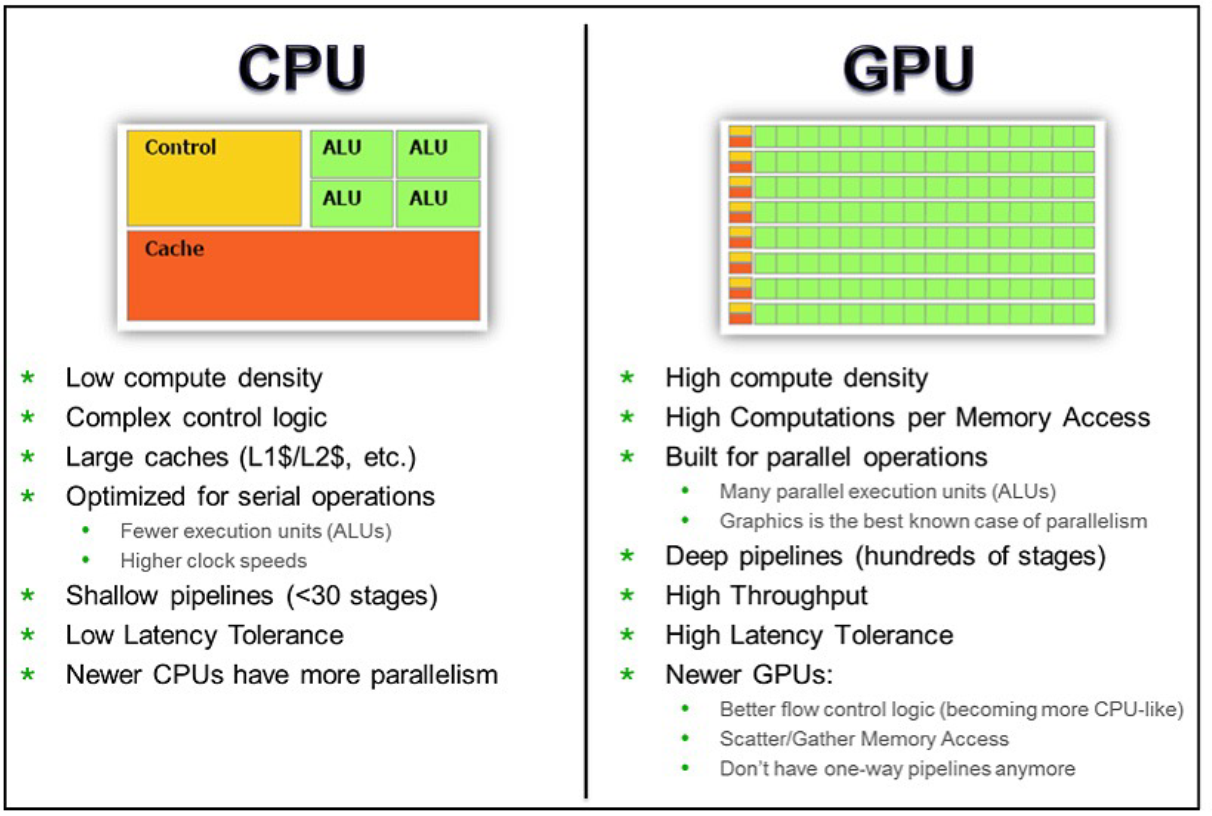
\includegraphics[width=0.4\textwidth]{img/img9.png}
    \caption{CPU vs GPU}
    \label{fig:CPU vs GPU}
    \end{center}
\end{figure}
The performance of such a synchronous system is limited by the slowest learner and slowest messages through the network. Since the communication phase is in the critical path, a high performance network can enable fast reconciliation of parameters across learners.\\
\textbf{GPUs within the rack: PCI AND NVlink}
GPUs are configured with a CPU host connected to a PCIe-attached accelerator tray with multiple GPUs.\\GPUs within the tray are connected using high-bandwidth interconnects such as NVlink.\\
\textbf{NVLINK evolution and NVSwitch}
In the A100 GPU, each NVLink lane supports a data rate of 50x 4 Gbit/s in each direction. The total number of NVLink lanes increases from six lanes in the V100 GPU to 12 lanes in the A100 GPU, now yielding 600 GB/s total
\subsubsection{Tensor Processing Unit (TPU)}
While suited to ML, GPUs are still relatively general purpose devices. In recent years, designers further specialized them to ML-specific hardware: Custom-built integrated circuit developed specifically for machine learning and tailored for TensorFlow.\\
\begin{multicols}{2}
    A Tensor is an n-dimensional matrix. This is the basic unit of operation in with TensorFlow.\\TPUs are used for training and inference:
\begin{itemize}
    \item TPUv1 is an inference-focused accelerator connected to the host CPU through PCIe links.
    \item Differently, TPUv2 and TPV3 focus training and inference
\end{itemize}
    Each Tensor core has an array for matrix computations (MXU) and a connection to high bandwidth memory (HBM) to store parameters and intermediate values during computation.
    \textbf{TPUv2}
    \\
    8 GiB of HBM for each TPU core, one MXU for each TPU core, 4 chips, 2 cores per chip.
    \columnbreak
    \noindent
    \begin{figure}[H]
        \begin{center}
        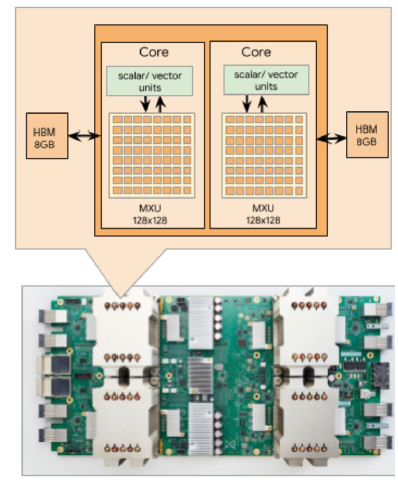
\includegraphics[width=0.28\textwidth]{img/img10.png}
        \caption{TPUv2 - 4 chips, 2 core per chip}
        \label{fig:TPUv2 - 4 chips, 2 core per chip}
        \end{center}
    \end{figure} 
\end{multicols}

In a rack multiple TPUv2 accelerator boards are connected through a custom high-bandwidth network to provide 11.5 petaflops of ML compute.\\
The high bandwidth network enables fast parameter reconciliation with well-controlled tail latencies.\\ Up to 512 total TPU cores and 4 TB of total memory in a TPU Pod (64 units).\\
\textbf{TPUv3} is the first \textbf{liquid-cooled accelerator}
in Google’s data center (here there is no fresh air to cool it down, used fresh liquid). 2.5x faster than TPUv2. Such supercomputing-class computational power supports new ML capabilities (e.g., AutoML), and rapid neural architecture search. The v3 TPU Pod provides a maximum configuration of 256 devices for a total 2048 TPU v3 cores, 100 petaflops and 32 TB of TPU memory.\\
\textbf{TPUv4} announced June 2021, used to support Google services (not yet available as a cloud service).One v4 TPU pod includes 4096 devices: About 2.7x faster than TPUv3 and same computing capacity as 10
millions of laptops. 


\subsubsection{Field-Programmable Gate Array (FPGA)}
Array of logic gates that can be programmed (“configured”) in the field, i.e.,by the user of the device as opposed to the people who designed it.\\ Array of carefully designed, and interconnected digital subcircuits, that efficiently implement common functions offering very high levels of flexibility. The digital subcircuits are called configurable logic blocks (CLBs).\\VHDL and Verilog are hardware description languages (HDLs), that allow to “describe” hardware. HDL code is more like a schematic that uses text to introduce components and create interconnections.\\Microsoft deployed FPGAs inside its Datacenters.
\begin{figure}[H]
    \begin{center}
    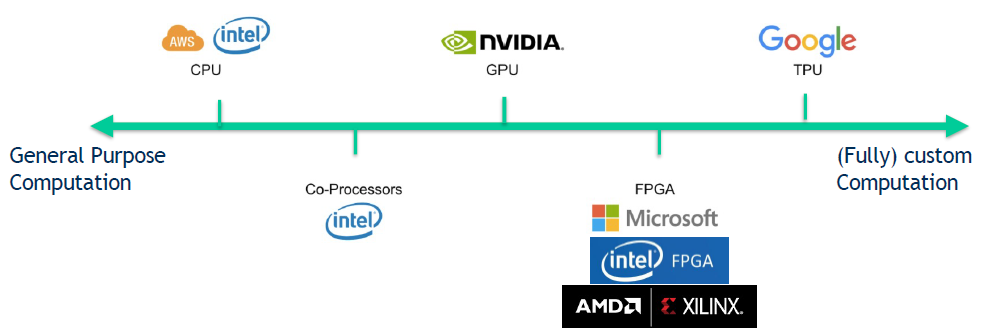
\includegraphics[width=0.4\textwidth]{img/img11.png}
    \caption{Overview}
    \label{fig:Overview}
    \end{center}
\end{figure}
\subsubsection{Advantages and Disadvantages}
\textbf{CPU}
\begin{itemize}
    \item {\bf Advantages}:Easy to be programmed and support any programming framework.\\ Fast design space exploration
    and run your applications.
    \item {\bf Disadvantages}: Most suited for simple AI models that do not take long to train and for small models with small training set.
\end{itemize}
\textbf{GPU}
\begin{itemize}
    \item {\bf Advantages}:Ideal for applications in which data need to be processed in parallel like the pixels of images or videos.
    \item {\bf Disadvantages}: Programmed in languages like CUDA and OpenCL and therefore provide limited flexibility compared to CPUs.
\end{itemize}
\textbf{TPU}
\begin{itemize}
    \item {\bf Advantages}:Very fast at performing dense vector and matrix computations and are specialized on running very fast program based on Tensorflow.
    \item {\bf Disadvantages}: For applications and models based on the TensorFlow. Lower flexibility compared to CPUs and GPUs.
\end{itemize}
\textbf{FPGA}
\begin{itemize}
    \item {\bf Advantages}:Higher performance, lower cost and lower power consumption compared to other options like CPUs and GPU.
    \item {\bf Disadvantages}: Programmed using OpenCL and High-level Synthesis (HLS).\\Limited flexibility compared to
    other platforms.
\end{itemize}
\newpage

%----------------------------------------%
\section{Storage}
Nowadays machines generate data at an unprecedented rate 


\begin{itemize}
        \item Disks and Flash SSDs are the building blocks of today’s WSC storage systems.
        \item These devices are connected to the data-center network and managed by sophisticated distributed systems
    \end{itemize} 
Examples: 
\begin{itemize}
    \item Direct Attached Storage (DAS)
    \item Network Attached Storage (NAS)
    \item Storage Area Networks (SAN)
    \item RAID controllers
\end{itemize}

\subsection{Hard Disk Drives}
\begin{multicols}{2}
A hard disk drive (HDD) is a data storage using rotating disks (platters) coated with magnetic material.\\
Data is read in a random-access manner, meaning individual blocks of data can be stored or retrieved in any order rather than sequentially.\\
An HDD consists of one or more rigid ("hard") rotating disks (platters) with magnetic heads arranged on a moving actuator arm to read and write data to the surfaces.\\
The {\bf Sector} is where you read and/or write; The organization of the data is in order to minimize the movement of the head (that increase the seek time): place the data that are related near! If the head continues to go forward and back increase the Latency!
\columnbreak
\begin{figure}[H]
    \begin{center}
    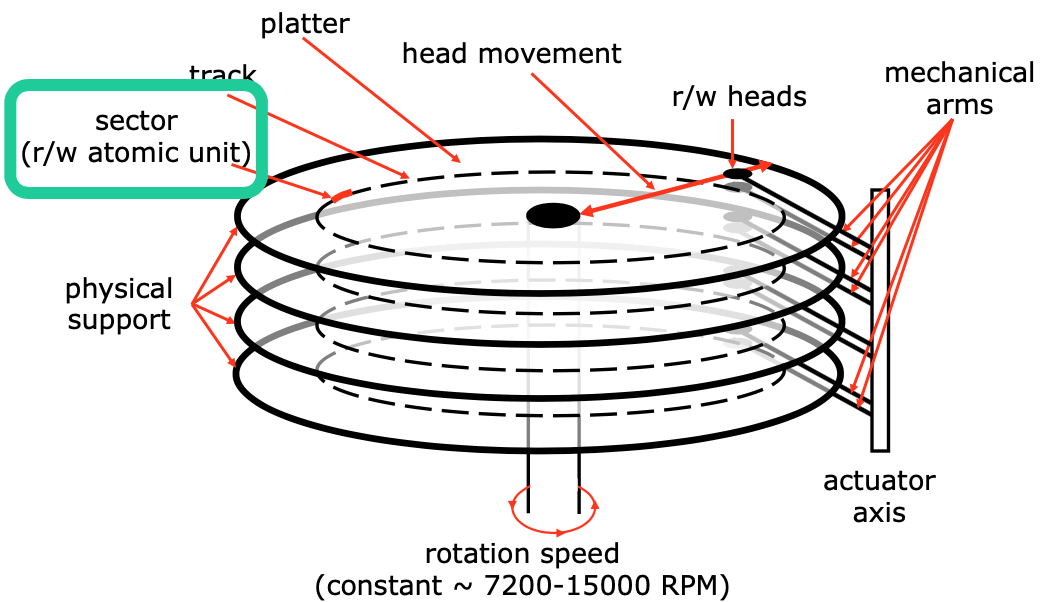
\includegraphics[width=0.5\textwidth]{img/img12.png}
    \caption{Hard Disk}
    \label{fig:HDD}
    \end{center}
\end{figure}
\end{multicols}
\subsubsection{Read Write heads, basic characteristic}
\begin{itemize}
    \item float on a film of air (tens of nanometers) above the platters
    \item one head for each magnetic platter
    \item cylinder: set of tracks with the same radius
    \item {\bf seek time}: time required to reach the track that contains the data, 3$\div$14 ms
\end{itemize}
\subsubsection{Other characteristics}
\begin{itemize}
    \item Diameter: about 9 cm (3,5$\div$2.5 in) - two surfaces
    \item Rotation speed: 7200$\div$15000 RPM round per minute
    \item Track density: 16,000 TPI (Track Per Inch)
    \item Sectors: 512 Byte (usually), but might be different (are numbered sequentially, have a header and an error correction code)
    \item Heads: can be parked close to the center or to the outer diameter (mobile drives)
    \item Disk buffer cache: embedded memory in a hard disk drive that has the function of a buffer between the disk and the computer (several MB)
\end{itemize}

\begin{figure}[H]
    \begin{center}
    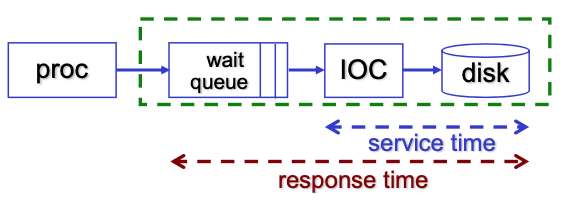
\includegraphics[width=0.5\textwidth]{img/img13.png}
    \caption{HDD service and response time}
    \label{fig:HDD time}
    \end{center}
\end{figure}
{\bf Service Time}\\
$s_{disk}$: seek time + rotational latency + data transfer time + controller overhead
\begin{itemize}
    \item {\bf seek} time: head movement time ($\approx$ ms), is a function of the number of cylinders traversed
    \item {\bf latency} time: time to wait for the sector ($\approx$ ms, $\frac{1}{2}$ round)
    \item {\bf transfer} time: is a function of rotation speed, storing density, cylinder position ($\approx$ MB/sec)
    \item {\bf controller overhead}: buffer management (data transfer) and interrupt sending time
\end{itemize}
no queue, average time to serve a single I/O request.
\newline
{\bf Response Time}\\
service time + queue time, average time to serve an I/O request in working conditions
\newline

\subsection{Solid-state Storage Device}
No mechanical or moving parts like HDD\\
Built out of transistors (like memory and processors)\\
Retain information despite power loss unlike typical RAM\\
A controller is included in the device with one or more solid state memory components\\
It uses traditional hard disk drive (HDD) interfaces (protocol and physical connectors) and form factors\\
Higher performance than HDD\\
It stores Bit, based on Transistors (which compose them):
\begin{multicols}{2}
\begin{itemize}
    \item Single-level cell (SLC) : single bit per cell 
    \item Multi-level cell (MLC) cell : two bits per cell
    \item Triple-level cell (TLC) : three bits per cell
    \item QLC, PLC...
\end{itemize}
\columnbreak
\noindent
\begin{figure}[H]
    \begin{center}
    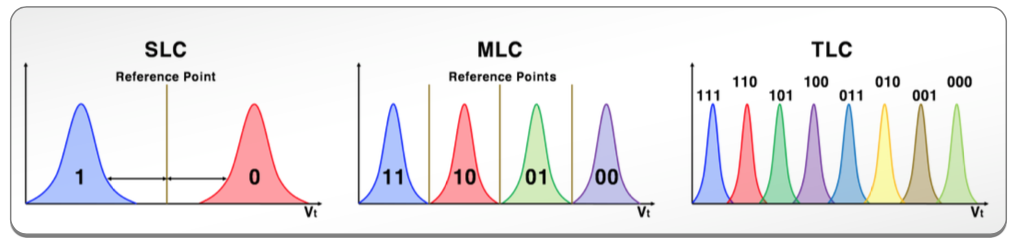
\includegraphics[width=0.5\textwidth]{img/img14.png}
    \caption{SSD}
    \label{fig:SSDs}
    \end{center}
\end{figure}
\end{multicols}
\subsubsection{Internal Organization}
NAND flash is organized into Pages and Blocks:\\
A {\bf page} contains multiple logical block (e.g. 512B-4KB) addresses (LBAs), a {\bf block} typically consists of multiple pages (e.g., 64) with a total capacity of around 128-256KB; Block/Page terminology in the SSD context can clash with previous use.\\
{\bf Blocks} (or Erase Block): smallest unit that can be erased. It consists of multiple pages and can be cleaned using the ERASE command.\\
{\bf Pages} : smallest unit that can be read/written. It is a sub-unit of an erase block and consists of the number of bytes which can be read/written in a single operations through the READ or PROGRAM commands.\\
Pages can be in three states:
\begin{itemize}
    \item Dirty (or INVALID): they contain data, but this data is no longer in use (or never used)
    \item Empty (or EREASED): they do not contain data
    \item In use (or VALID): the page contains data that can be actually read
\end{itemize}
Only empty pages can be written\\
Only dirty pages can be erased, but this must be done at the block
level (all the pages in the block must be dirty or empty)\\
It is meaningful to read only pages in the “in use” (“valid”) state\\
If no empty page exists, some dirty page must be erased:
\begin{itemize}
    \item If no block containing just dirty or empty pages exists, then special procedures should be followed to gather empty pages over the disk
    \item To erase the value in flash memory the original voltage must be reset to neutral before a new voltage can be applied, known as write amplification
\end{itemize}
{\bf Remark: we can write and read a single page of data from a SSD but we have to delete an entire block to release it}\\
\newline
{\bf WRITE AMPLIFICATION}: the actual amount of information physically written to the storage media is a multiple of the logical amount intended to be written.\\
\newline
{\bf Wear out}: breakdown of the oxide layer within the floating-gate transistors of NAND flash memory.\\
The erasing process hits the flash cell with a relatively large charge of electrical energy.\\
Each time a block is erased:
\begin{itemize}
    \item the large electrical charge actually degrades the silicon material
    \item after enough write-erase cycles, the electrical properties of the flash cell begin to break down and the cell becomes unreliable
\end{itemize}
{\bf Flash Translation Layer} = layer that matches the file system and the SSD.\\
\begin{multicols}{2}
\begin{figure}[H]
    \begin{center}
    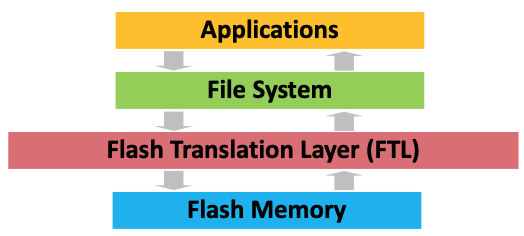
\includegraphics[width=0.5\textwidth]{img/img15.png}
    \caption{Flash Translation Layer}
    \label{fig:FTL}
    \end{center}
\end{figure}
\columnbreak
Direct mapping between Logical to Physical pages is not feasible\\
FTL is an SSD component that make the SSD “look as HDD”:
\begin{enumerate}
    \item Data Allocation and Address translation
    \begin{itemize}
        \item Efficient to reduce Write Amplification effects
        \item Program pages within an erased block in order (from low to high pages): Log-Structured FTL
    \end{itemize}
    \item Garbage collection: Reuse of pages with old data (Dirty/Invalid)
    \item  Wear leveling: FTL should try to spread writes across the blocks of the flash ensuring that all of the blocks of the device wear out at roughly the same time
\end{enumerate}
\end{multicols}

{\bf Garbage collection}\\
When an existing page is updated à old data becomes obsolete!\\
Old version of data are called garbage and (sooner or later) garbage pages must be reclaimed for new writes to take place.\\
Garbage Collection is the process of finding garbage blocks and reclaiming them: Simple process for fully garbage blocks or more complex for partial cases. I.e. Basic steps: 
\begin{enumerate}
    \item Find a suitable partial block
    \item Copy non-garbage pages
    \item Reclaim (erase) the entire block for writing
\end{enumerate}
\begin{figure}[H]
    \begin{center}
    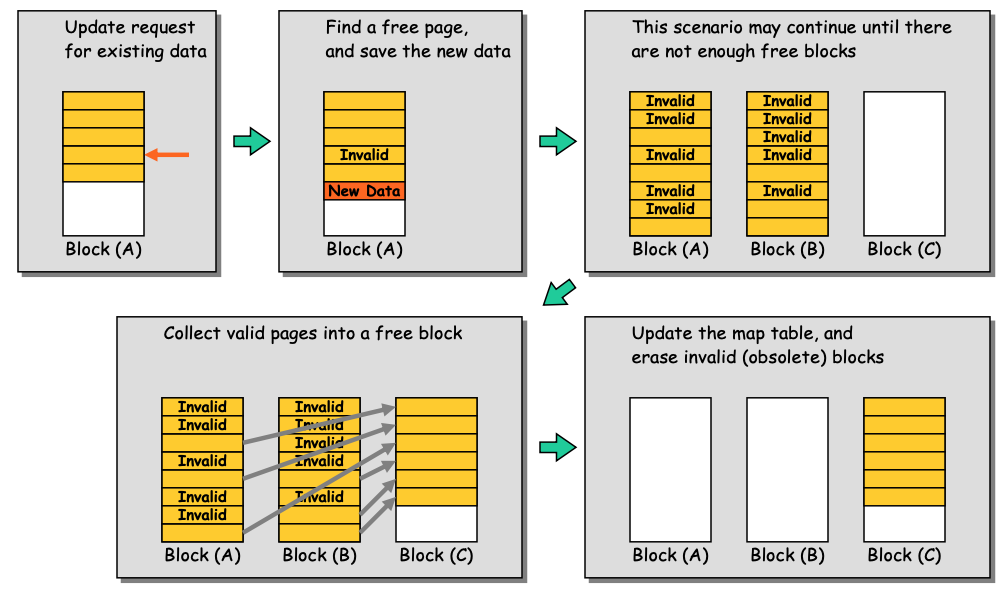
\includegraphics[width=0.4\textwidth]{img/img16.png}
    \caption{Garbage collection (Example)}
    \label{fig:GC ex}
    \end{center}
\end{figure}
Garbage collection is expensive: Require reading and rewriting of live data and the ideal garbage collection is reclamation of a block that consists of only dead pages.\\
The {\bf8cost} of Garbage Collection depends on the amount of data blocks that have to be migrated.\\
Solutions to alleviate the problem:
\begin{itemize}
    \item Overprovision the device by adding extra flash capacity: Cleaning can be delayed
    \item Run the Garbage Collection in the background using less busy periods for the disk
\end{itemize}
When performing background GC the SSD assumes to know which pages are invalid\\
{\bf Problem}: most file systems don’t actually delete data (E.g., on Linux, the “delete” function is unlink() and it removes the file meta-data, but not the file itself)
\begin{figure}[H]
    \begin{center}
    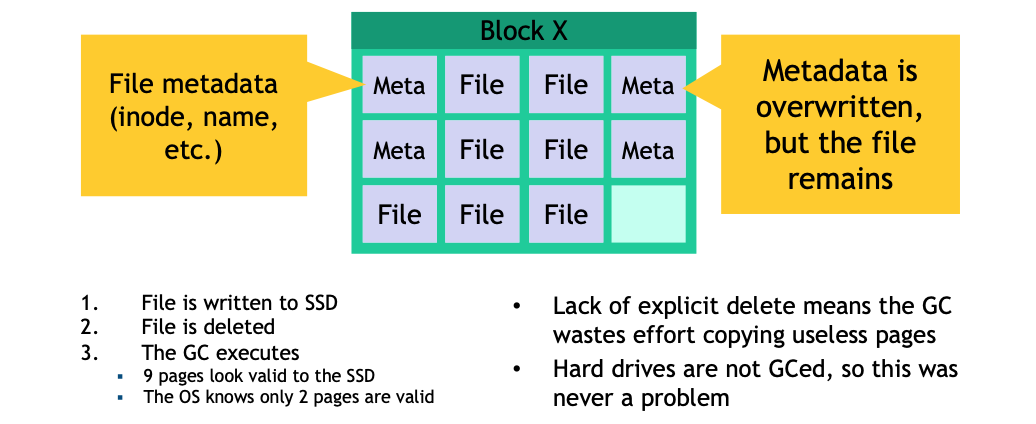
\includegraphics[width=0.8\textwidth]{img/img17.png}
    \caption{Garbage collection (Example)}
    \label{fig:GC ex}
    \end{center}
\end{figure}
New SATA command TRIM (SCSI – UNMAP): The OS tells the SSD that specific LBAs are invalid and may be GCed.\\
OS support for TRIM (Win 7, OSX Snow Leopard, Linux 2.6.33, Android 4.3).\\
\newline
The size of page-level mapping table is too large:
With a 1TB SSD with a 4byte entry per 4KB page, 1GB of is needed for mapping.\\
Some approaches to reduce the costs of mapping:
\begin{itemize}
    \item \underline{Block-based mapping}: Coarser grain approach.\\
    Mapping at block granularity, to reduce the size of a mapping table. Small write problem: the FTL must read a large amount of live data from the old block and copy them into a new one.
    \item \underline{Hybrid mapping} : Multiple tables.\\
    FTL maintains two tables:
    \begin{itemize}
        \item Log blocks: page mapped
        \item Data blocks: block-mapped
    \end{itemize}
    When looking for a particular logical block, the FTL will consult the page mapping table and block mapping table in order
    \item \underline{Page mapping plus caching} : Exploiting Data Locality.\\
    Basic idea is to cache the active part of the page-mapped FTL, f a given workload only accesses a small set of pages, the translations of those pages will be stored in the FTL memory. High performance without high memory cost if the cache can contain the necessary working set. Cache miss overhead. exists
\end{itemize}
{\bf Wear Leveling}\\
Erase/Write cycle is limited in Flash memory:\\
- Skewness in the EW cycles shortens the life of the SSD\\
- All blocks should wear out at roughly the same time\\
Log-Structured approach and garbage collection helps in spreading writes. However, a block may consist of cold data 
\begin{itemize}
    \item the FTL must periodically read all the live data out of such blocks and re-write it elsewhere
    \item Wear leveling increases the write amplification of the SSD and decreases performance (Simple Policy: Each Flash Block has EW cycle counter, Maintain |Max(EW cycle) – Min(EW cycle)|$<$ e)
\end{itemize}

\subsubsection{SSD summary}
\begin{itemize}
    \item They cost more than the conventional HDD
    \item Flash memory can be written only a limited number of times (wear):\\
    have a shorter lifetime\\
    error correcting codes\\
    over-provisioning (add some spare capacity)
    \item Different read/write speed\\
    Write amplification
    \item Write performance degrades of one order of magnitude after the first writing
    \item Often the controller become the real bottleneck to the transfer rate
    \item SSD are not affected by data-locality and must not be defragmented (actually, defragmentation may damage the disks)
    \item Flash Translation Layer is one of the key components\\
    - Data Allocation\\
    - Address Translation\\
    - Garbage Collection\\
    - Wear Leveling
\end{itemize}

\subsection{HDD vs SSD}
\begin{multicols}{2}
{\bf Unrecoverable Bit Error Ratio} (UBER): A metric for the rate of occurrence of data errors, equal to the number of data errors per bits read\\ 
{\bf Endurance rating} : Terabytes Written (TBW is the total amount of data that can be written into an SSD before it is likely to fail). The number of terabytes that may be written to the SSD while still meeting the requirements\\
\columnbreak
\begin{figure}[H]
    \begin{center}
    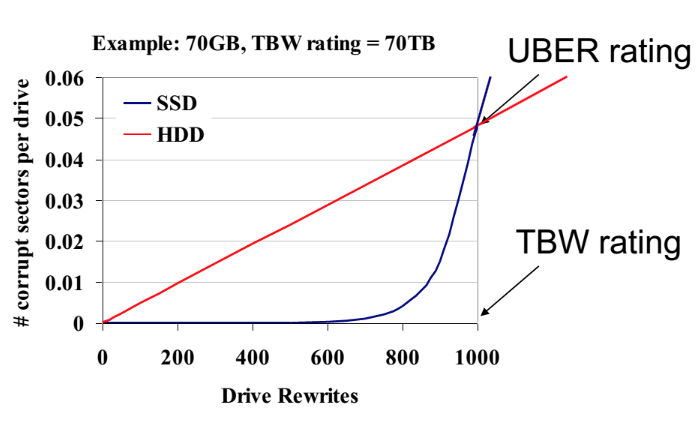
\includegraphics[width=0.3\textwidth]{img/img18.png}
    \caption{Garbage collection (Example)}
    \label{fig:GC ex}
    \end{center}
\end{figure}
\end{multicols}
Memory cells can accept data recording between 3,000 and 100,000 during its lifetime: once the limit value is exceeded, the cell "forgets" any new data\\
\newline
A typical TBW for a 250 GB SSD is between 60 and 150 Terabytes of data written to the drive; This means that in order to overcome, for example, a TBW of 70 Terabytes, a user should write 190 GB every day for a year or fill his SSD on a daily basis for two thirds with new files for a whole year\\
\newline
It is difficult to comment on the duration of SSDs: Dell, in an old study (2011), spoke of an estimated duration between three months and ten years explaining, however, that there are so many factors (temperature and workload) that may depend on the life of an SSD that is very difficult to make predictions.

\subsection{Hybrid solution}
HDD + SSD
\begin{itemize}
    \item Some large storage servers use SSD as a cache for several HDD. Some mainboards of the latest generation have the same feature: they combine a small SSD with a large HDD to have a faster disk.
    \item Some HDD manufacturers produce Solid State Hybrid Disks (SSHD) that combine a small SDD with a large HDD in a single unit.
\end{itemize}


\subsection{Storage system}
\begin{multicols}{2}
\begin{figure}[H]
    \begin{center}
    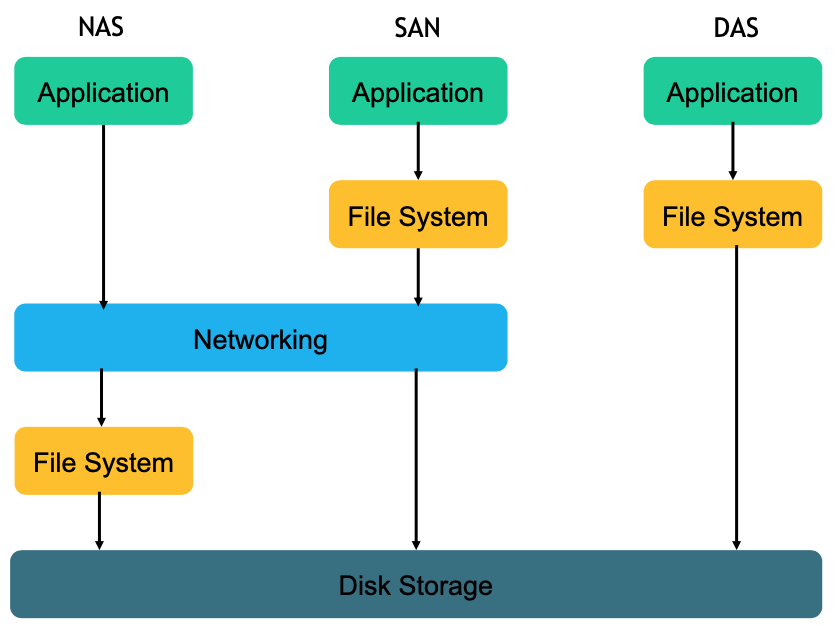
\includegraphics[width=0.4\textwidth]{img/img19.png}
    \caption{NAS SAN DAS}
    \label{fig:NAS SAN DAS}
    \end{center}
\end{figure}
\columnbreak
\begin{defn}
A {\bf Direct Attached Storage} (DAS) is a storage system directly attached to a server or workstation. They are visible as disks/volumes by the client OS.
\end{defn}
\begin{defn}
A {\bf Network Attached Storage} (NAS) is a computer connected to a network that provides only file-based data storage services (e.g., FTP, Network File System and SAMBA) to other devices on the network and is visible as File Server to the client OS
\end{defn}
\begin{defn}
{\bf Storage Area Networks} (SAN) are remote storage units that are connected to a server using a specific networking technology (e.g., Fiber Channel) and are visible as disks/volumes by the client OS
Direct Attached Storage (DAS) is a storage system directly
\end{defn}
\end{multicols}



\subsubsection{DAS}
DAS is a storage system directly attached to a server or workstation\\
The term is used to differentiate non-networked storage from SAN and NAS (that will be described later).\\
{\bf Main features}:
\begin{itemize}
    \item limited scalability (for ex. if I want 100 server connected, I have to multiply x100 the capacity)
    \item complex management
    \item to read files in other machines, the “file sharing” protocol of the OS must be used (on application laver, if I have one Windows and one Linux they must be able to communicate)
\end{itemize}
{\bf Internal and external}:
\begin{itemize}
    \item DAS does not necessary mean “internal drives” (it could have an external hard disk)
    \item All the external disks, connected with a point-to-point protocol to a PC can be considered as DAS
\end{itemize}

\subsubsection{NAS}
A NAS unit is a computer connected to a network that provides only file-based data storage services to other devices on the network.\\
NAS systems contain one or more hard disks, often organized into logical redundant storage containers or RAID.\\
Provide file-access services to the hosts connected to a TCP/IP network though Networked File Systems/SAMBA.\\
Each NAS element has its own IP address.\\
Good scalability (incrementing the devices in each NAS element
or incrementing the number of NAS elements).\\
\newline
{\bf NAS vs DAS}\\
The key differences between direct-attached storage (DAS) and NAS are:
\begin{itemize}
    \item DAS is simply an extension of an existing server and is not necessarily networked
    \item NAS is designed as an easy and self-contained solution for sharing files over the network
\end{itemize}
Comparing NAS with local (non-networked) DAS, the {\sl performance} of NAS depends mainly on the speed of and congestion on the network

\subsubsection{SAN}
Storage Area Networks, are remote storage units that are connected to a PC/server using a specific networking technology.\\
SANs have a special network devoted to the accesses to storage devices.\\
Two distinct networks (one TCP/IP and one dedicated network, e.g., Fber Channer).\\
High scalability (simply increasing the storage devices connected to the SAN network).\\
\newline
{\bf NAS vs SAN}\\
\begin{itemize}
    \item NAS provides both storage and a file system
    \item This is often contrasted with SAN which provides only block-based storage and leaves file system concerns on the "client" side
    \item One way to loosely conceptualize the difference between a NAS and a SAN is that:
    \begin{itemize}
        \item NAS appears to the client OS (operating system) as a file server (the client can map network drives to shares on that server)
        \item a disk available through a SAN still appears to the client OS as a disk: it will be visible in the disks and volumes management utilities (along with client's local disks), and available to be formatted with a file system
    \end{itemize}
    \item NAS is used for low-volume access to a large amount of storage by many users
    \item SAN is the solution for petabytes (1012) of storage and multiple, simultaneous access to files, such as streaming audio/video
\end{itemize}

\begin{figure}[H]
    \begin{center}
    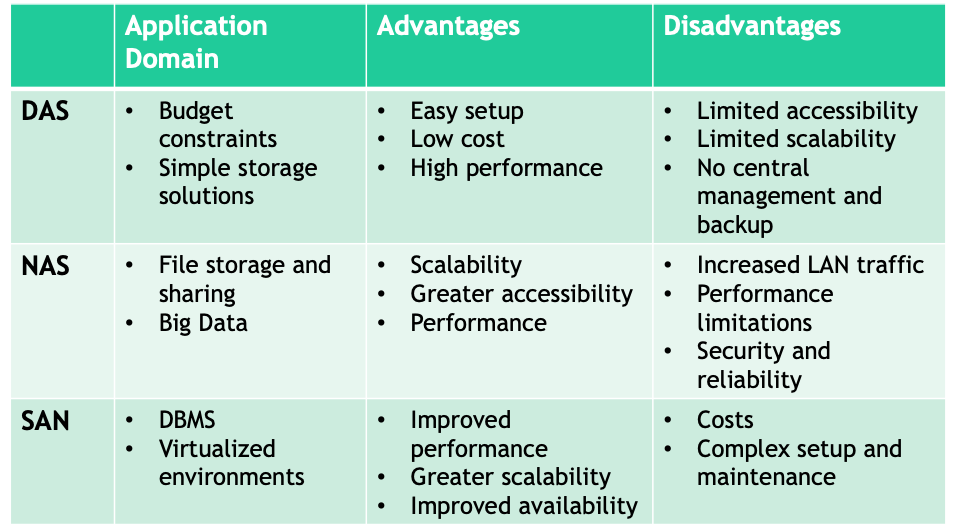
\includegraphics[width=0.5\textwidth]{img/img20.png}
    \caption{NAS vs SAN vs DAS}
    \label{fig:NAS,SAN,DAS}
    \end{center}
\end{figure}

\newpage

%------------------------------------------------------%
\section{Networking}
{\sl Communication} equipment allows network interconnections among the devices.\\
They can be:
\begin{itemize}
    \item Hubs
    \item Routers
    \item DNS or DHCP servers
    \item Load balancers
    \item Technology switches
    \item Firewalls
\end{itemize}
The performance of servers increases over time, the demand for inter-server bandwidth naturally increases as well!\\
{\sl We can double the aggregate compute capacity or the aggregate storage simply by doubling the number of compute or storage elements}, but how?\\
Networking has no straightforward horizontal scaling solution.\\
Doubling leaf bandwidth is easy: with twice as many servers, we’ll have twice as many network ports and thus twice as much bandwidth.
\begin{multicols}{2}
\noindent
But if we assume that every server needs to talk to every other server, we need to deal with {\bf bisection bandwidth}. \begin{defn}The bandwidth across the narrowest line that equally divides the cluster into two parts. Characterizes network capacity since randomly communicating processors must send data across the “middle” of the network
\end{defn}
\columnbreak
\begin{figure}[H]
    \begin{center}
    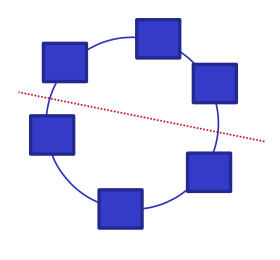
\includegraphics[width=0.2\textwidth]{img/img21.png}
    \caption{bisection bandwidth}
    \label{fig:bisection bandwidth}
    \end{center}
\end{figure}
\end{multicols}
\subsection{Architecture}
\begin{figure}[H]
    \begin{center}
    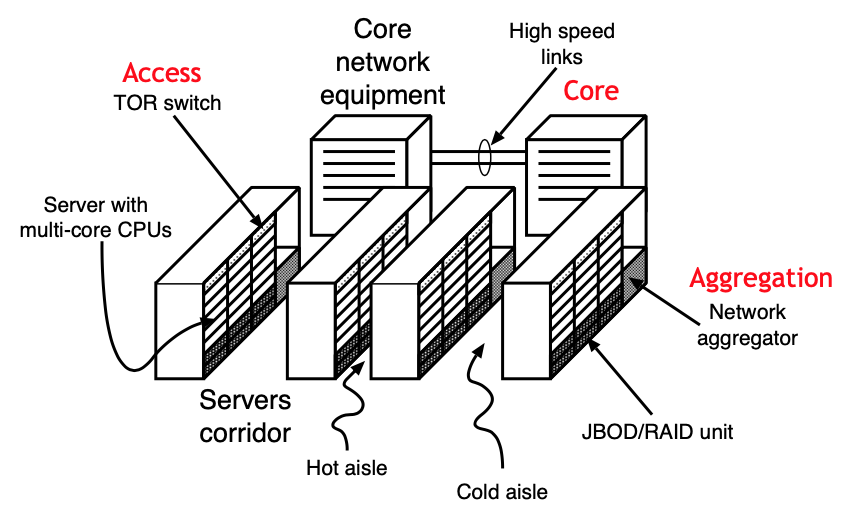
\includegraphics[width=0.4\textwidth]{img/img22.png}
    \caption{Data-center network architectures}
    \label{fig:DS net architecture}
    \end{center}
\end{figure}
Switches at the access layer can be put into two positions:
\begin{itemize}
    \item {\sl Top-Of-the-Rack} (TOR): {\bf Access} switches are put at the top of each rack. The number of cables is limited. The number of ports per switch is also limited (lower costs). However, the scalability is also limited.
    \item {\sl End-Of-the-Line} (EOL): Switches are positioned one per corridor, at the end of a line of rack. {\bf Aggregation} switches must have a larger number of ports, and longer cables are required (higher costs). However, the system can scale to have a larger number of machines.
\end{itemize}
Three layer architecture configures the network in three different
layers:
\begin{itemize}
    \item core
    \item aggregation
    \item access
\end{itemize}
{\bf Bandwidth} can be increased by increasing the switches at the core and aggregation layers, and by using routing protocols such as Equal Cost Multiple Path (ECMP) that equally shares the traffic among different routes.\\
\newline
This solution is very simple, but can be very expensive in large data-centers since:\\
• Upper layers require faster network equipments. (For example: 1 GB Ethernet at the access layer, 10 GB Ethernet at the aggregation layer, 25 GB Optical connections at the core layer)\\
• The cost in term of acquisition and energy consumption can be very high\\
{\sl Another benefit of SANs: a way to tackle network scalability, offload some traffic to a special-purpose network connecting servers to storage units
}
\begin{multicols}{2}
    \begin{figure}[H]
        \begin{center}
        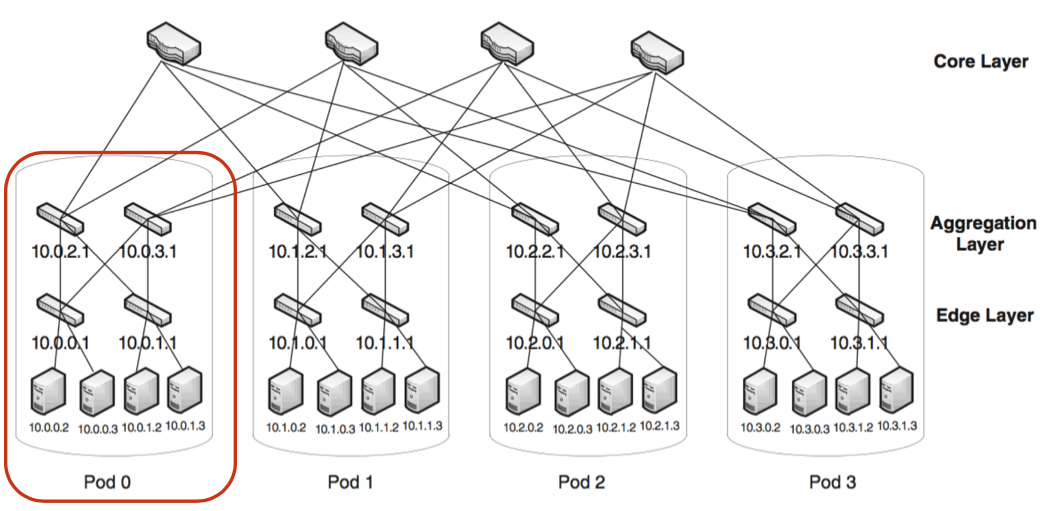
\includegraphics[width=0.3\textwidth]{img/img23.png}
        \caption{Fat-tree topologies}
        \label{fig:Fat-tree topologies}
        \end{center}
    \end{figure}
Fat-tree topologies use a larger number of slower speed switches and connections. In particular, nodes are divided into pods characterized by the same number of nodes and switches.
    \columnbreak
    \begin{figure}[H]
        \begin{center}
        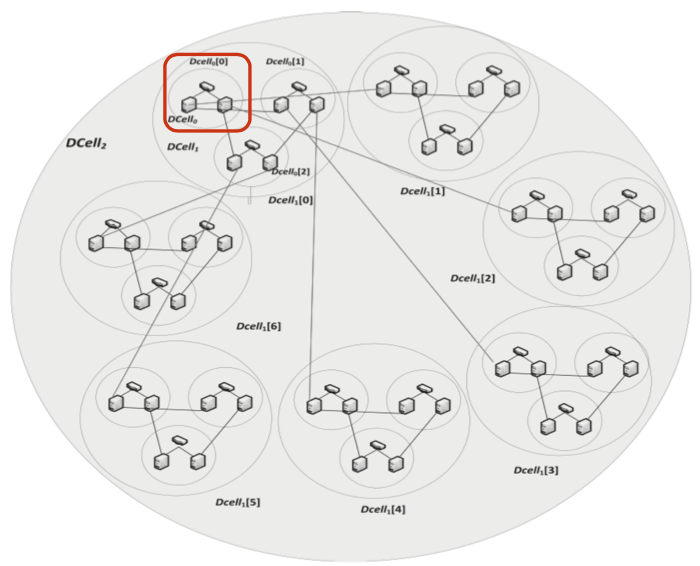
\includegraphics[width=0.2\textwidth]{img/img24.png}
        \caption{D-Cell topology}
        \label{fig:D-Cell topology}
        \end{center}
    \end{figure}
D-Cell topology, defines the network in recursive way. Cells are organized in levels. Switches connects nodes at the lower level.Some nodes belong to different cells: they perform routing among them to create a higher level cell. 
\end{multicols}
\subsubsection{High Performance Clusters}
High-Performance Computing (HPC) supercomputer clusters often have a much lower ratio of computation to network bandwidth.\\
\newline
Applications (e.g., weather simulations) distribute their data across RAM in all nodes, and nodes need to update neighboring nodes after performing relatively few floating-point computations.\\
Traditional HPC systems have used proprietary interconnects with leading-edge link bandwidths, much lower latencies, and some form of a global address space (where the network is integrated with CPU caches and virtual addresses)\\
\newline
High {\bf throughputs} but much more expensive solutions.
\subsection{Network to support Virtualization}
Connection endpoints (i.e., IP address/port combinations) can move from one physical machine to another\\ 
Typical networking hardware as well as network management software don’t anticipate such moves and in fact often explicitly assume that they’re not possible \\ (All machines in a given rack have IP addresses in a common subnet, which simplifies administration and minimizes the number of required forwarding table entries routing tables)\\ \underline{Solution}: the cluster manager that decides the placement of computations also updates the network state through programmable Network control planes (Software Defined Networks)
\subsection{The interplay of storage and networking technology}
The success of WSC distributed storage systems can be partially attributed to the evolution of data center networking fabrics:{\sl disk locality is no longer relevant in intra-data center computations}.\\
This observation enables:
\begin{itemize}
    \item simplifications in the design of distributed disk-based storage
    systems
    \item utilization improvements
\end{itemize}since any disk byte in a WSC facility can, in principle, be utilized by any task regardless of their relative locality
\subsection{Balanced design}
{\sl  Computer architects are trained to solve the problem of finding the right combination of performance and capacity from the various building blocks that make up a WSC}\\ \\
The right building blocks are apparent only when one considers the entire WSC system.\\
It is important to characterize the kinds of workloads that will execute on the system with respect to their consumption of various resources.\\
Keeping in mind three important considerations:
\begin{enumerate}
    \item Smart programmers may be able to restructure their algorithms to
    better match a more inexpensive design alternative
    \item The most cost-efficient and balanced configuration for the hardware may be a match with the combined resource requirements of multiple workloads
    \item Fungible resources tend to be more efficiently used
\end{enumerate}
System balance: {\bf Storage Hierarchy}
\subsubsection*{Example}
\begin{multicols}{2}
We assume a system with 5,000 servers, each with 256 GB of DRAM, one 4 TB SSD, and eight 10 TB disk drives.\\
Each group of 40 servers is connected through a 40-Gbps link to a rack-level switch (TOR)\\
Each rack has an additional 10-Gbps uplink bandwidth per machine for connecting the rack to the cluster-level switch (AGGREGATION)\\
Network latency numbers assume a TCP/IP transport, and networking bandwidth values assume that each server is using its fair share of the available cluster-level bandwidth.\\
For disks, typical commodity disk drive (SA T A) latencies and transfer rates are considered.
\columnbreak
\begin{figure}[H]
    \begin{center}
    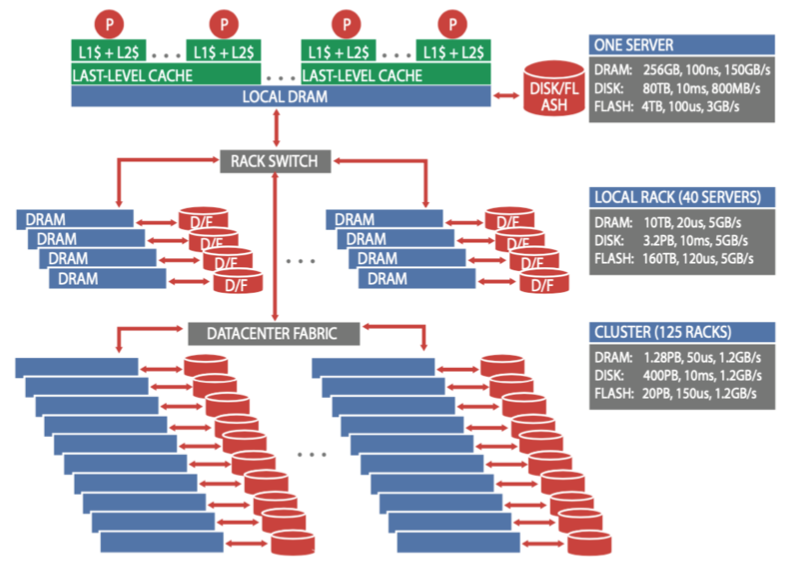
\includegraphics[width=0.4\textwidth]{img/img25.png}
    \caption{Storage Hierarchy}
    \label{fig:Storage Hierarchy}
    \end{center}
\end{figure}
\end{multicols}
A large application that requires servers in many racks to operate must deal effectively with large discrepancies in latency, bandwidth, and capacity.\\
\newline
These discrepancies are much larger than those seen on a single machine, making it more difficult to program a WSC:
\begin{itemize}
    \item A key challenge for architects of WSCs is to smooth out these discrepancies in a cost-efficient manner
    \item A key challenge for software architects is to build SW infrastructure and services that hide this complexity
\end{itemize} Three specific comments about SSDs:
\begin{enumerate}
    \item Much faster than HDDs
    \item Demand a high bandwidth
    \item In the worst case, writes to flash can be several orders of magnitude slower than reads
\end{enumerate}

\newpage
%------------------------------------------------------%

\section{Building and Infrastructures}
\begin{figure}[H]
    \begin{center}
    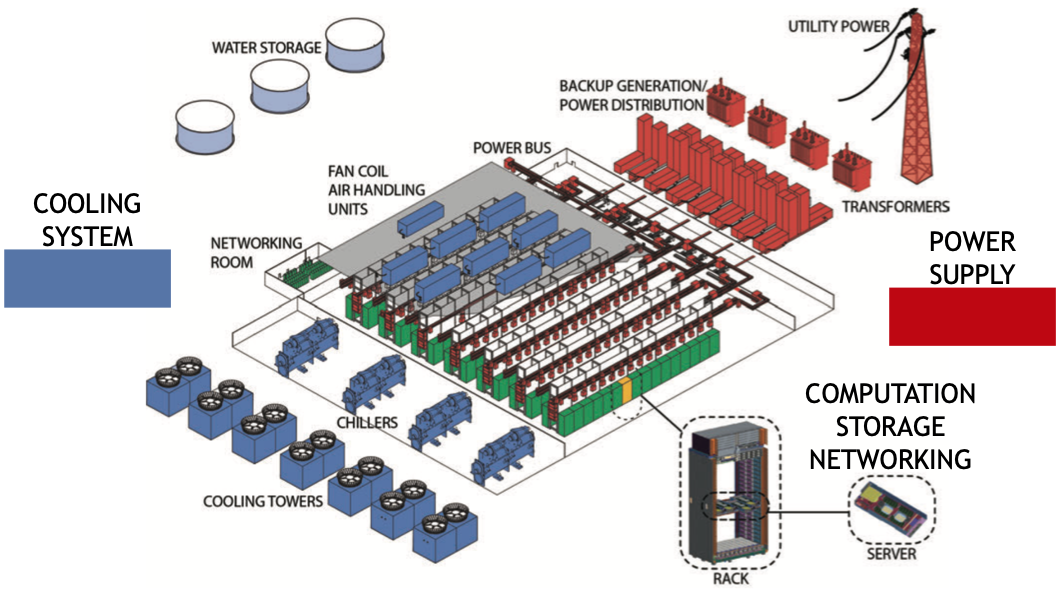
\includegraphics[width=0.7\textwidth]{img/img26.png}
    \caption{Main components of a typical data center}
    \label{fig:Main components}
    \end{center}
\end{figure}
WSC has not just computation, storage and networking; it has other important components related to power delivery, cooling, and building infrastructure that also need to be considered.
\subsection{Power System}
In order to protect against power failure, battery and diesel generators are used to backup the external supply.\\ \\
The UPS typically combines three functions in one system:
\begin{enumerate}
    \item contains a transfer switch that chooses the active power input (either utility power or generator power)
    \item contains some form of energy storage (electrical, chemical, or mechanical) to bridge the time between the utility failure and the availability of generator power
    \item conditions the incoming power feed, removing voltage spikes or sags, or harmonic distortions in the AC feed
\end{enumerate}
\subsection{Cooling System}
IT equipment generates a lot of heat: the cooling system is usually a very expensive component of the datacenter, and it is composed by coolers, heat-exchangers and cold water tanks.
\subsubsection{Open-Loop}
The simplest topology is fresh air cooling (or air economization)— essentially, opening the windows. This is a single «open-loop» system.
\begin{defn}
    Free cooling, i.e., open-loop, refers to the use of cold outside air to either help the production of chilled water or directly cool servers. It is not completely free in the sense of zero cost, but it involves very low-energy costs compared to chillers. 
\end{defn}
\subsubsection{Closed-Loop}
\begin{defn}
    Closed-loop systems come in many forms, the most common being the air circuit on the data center floor.
\end{defn}
The goal is to isolate and remove heat from the servers and transport it to a heat exchanger.\\ Cold air flows to the servers, heats up, and eventually reaches a heat exchanger to cool it down again for the next cycle through the servers.
\begin{multicols}{2}
\begin{figure}[H]
    \begin{center}
    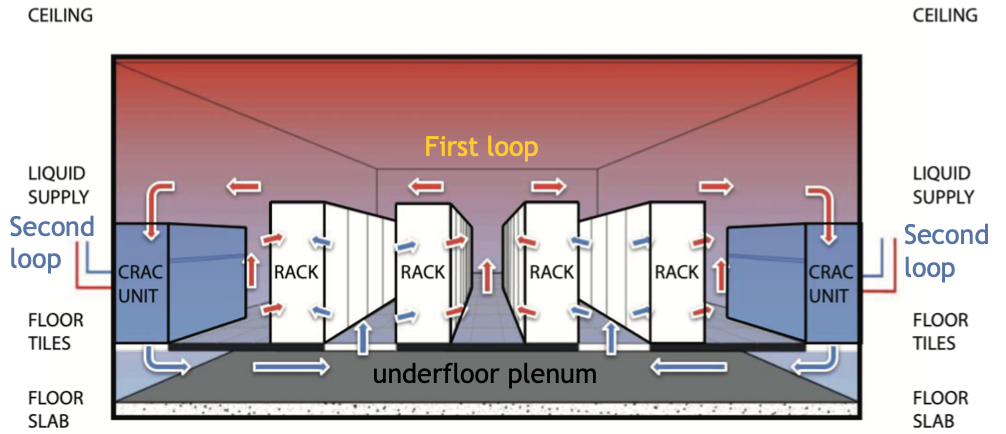
\includegraphics[width=0.5\textwidth]{img/img27.png}
    \caption{Closed-loop with two loop}
    \label{fig:Closed-loop with two loop}
    \end{center}
\end{figure}
\columnbreak
\subsubsection*{Closed-loop with two loops}
\begin{itemize}
    \item The airflow through the underfloor plenum, the racks, and back to the CRAC (a 1960s term for computer room air conditioning) defines the primary air circuit, i.e., the {\bf first loop}.
    \item The {\bf second loop} (the liquid supply inside the CRACs units) leads directly from the CRAC to external heat exchangers (typically placed on the building roof) that discharge the heat to the environment.
\end{itemize}
\end{multicols}
\subsubsection*{A three-loop system commonly used in large-scale data center}
\begin{figure}[H]
    \begin{center}
    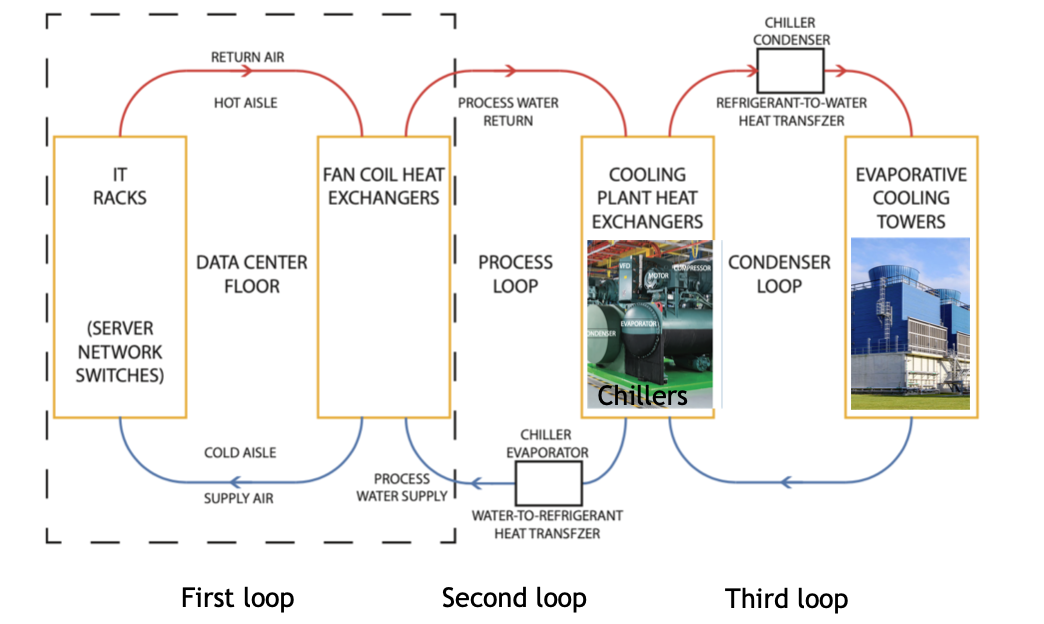
\includegraphics[width=0.4\textwidth]{img/img28.png}
    \caption{Closed-loop with three loop}
    \label{fig:Closed-loop with three loop}
    \end{center}
\end{figure}
A water-cooled {\bf chiller} can be thought of as a water-cooled air conditioner.\\
\newline
{\bf Cooling towers} cool a water stream by evaporating a portion of it into the atmosphere. They do not work as well in very cold climates because they need additional mechanisms to prevent ice formation
\subsubsection{Comparison}
Each topology presents tradeoffs in complexity, efficiency, and cost:
\begin{itemize}
    \item Fresh air cooling can be very efficient but does not work in all climates, requires filtering of airborne particulates, and can introduce complex control problems.
    \item Two-loop systems are easy to implement, relatively inexpensive to construct, and offer isolation from external contamination, but typically have lower operational efficiency.
    \item A three-loop system is the most expensive to construct and has moderately complex controls, but offers contaminant protection and good efficiency.
\end{itemize}
\subsubsection{In-rack cooling}
In-rack cooler adds an air-to-water heat exchanger at the back of a rack so the hot air exiting the servers immediately flows over coils cooled by water, essentially reducing the path between server exhaust and CRAC input
\subsubsection{In-row cooling}
In-row cooling works like in-rack cooling except the cooling coils are not in the rack, but adjacent to the rack.
\subsubsection{Liquid cooling}
We can directly cool server components using \underline{cold plates}, i.e., local liquid-cooled heat sinks:
\begin{itemize}
    \item Impractical to cool all compute components with cold plates.
    \item Components with the highest power dissipation are targeted
    for liquid cooling while other components are air-cooled.
\end{itemize}
The liquid circulating through the heat sinks transports the heat to a liquid-to-air or liquid-to-liquid heat exchanger that can be placed close to the tray or rack, or be part of the data center building (such as a cooling tower).
\subsubsection*{Container-based}
Container-based data centers go one step beyond in-row cooling by placing the server racks inside a container (typically 6 to 12 mt long) and integrating heat exchange and power distribution into the container as well.

\subsection{Power consumption}
Data-center power consumption is an issue, since it can reach several MWs.\\
Cooling usually requires about half the energy required by the IT equipment (servers + network + disks).\\
Energy transformation creates also a large amount of energy wasted for running a datacenter.\\
\begin{itemize}
    \item DCs consume 3\% of global electricity supply (416.2 TWh > UK’s 300 TWh).
    \item DCs produce 2\% of total greenhouse gas emissions (same as worldwide air traffic pre-pandemic).
    \item DCs produce as much CO2 as The Netherlands or Argentina.
\end{itemize}
\begin{figure}[H]
    \begin{center}
    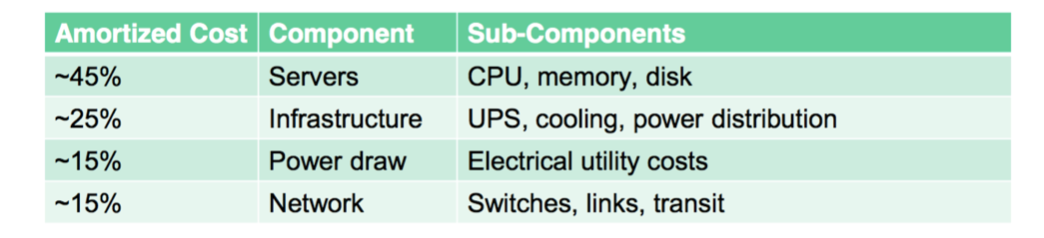
\includegraphics[width=0.6\textwidth]{img/img29.png}
    \caption{power consumption}
    \label{fig:power consumption}
    \end{center}
\end{figure}
\begin{defn}
    {\bf Power usage effectiveness} (PUE) is the ratio of the total amount of energy used by a DC facility to the energy delivered to the computing equipment
\end{defn}
PUE = $\frac{Total Facility Power}{IT Equipment power}$ 
\newline\newline
{\bf Total facility power} = covers IT systems (servers, network, storage) + other equipment (cooling, UPS, switch gear, generators, lights, fans, etc.)\\
{\bf Data Center infrastructure Efficiency} (DCiE): PUE inverse
\newline\newline

\subsection{Tiers}
Data-center availability is defined by in four different tier level. Each one has its own requirements.
\begin{figure}[H]
    \begin{center}
    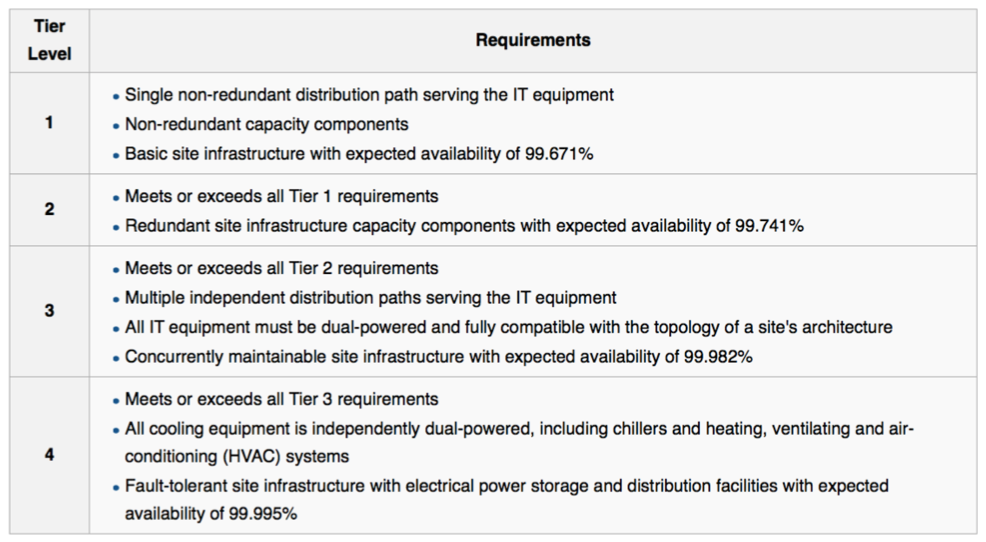
\includegraphics[width=0.6\textwidth]{img/img30.png}
    \caption{data-center tiers}
    \label{fig:tiers}
    \end{center}
\end{figure}

\newpage
%------------------------------------------------------------------%

\end{document}
